% ================================================================
% The Retrieve and Connect version of latex/starters/retrieval/lessPriorKnowledge/geometryBasedStarters4Qs_workedSolutions.tex
%
% This is the same deck as the one above, made by renaming the titles in it.
% Every slide that was a numbered starter is now titled
% "Retrieve and Connect", and the word is renamed wherever else a title
% used it. Nothing outside a title has been changed.
%
%   made from           latex/starters/retrieval/lessPriorKnowledge/geometryBasedStarters4Qs_workedSolutions.tex
%   retitling rules     version 1
%
% Please don't edit this file. It is written again from the one it was
% made from whenever that changes, so an edit here would be lost - edit
% that file instead and this one follows.
% ================================================================
% Root file used ashow macros
\documentclass[aspectratio=169]{beamer}
\usepackage{amsmath}
\usepackage{tikz}
\usetikzlibrary{angles,quotes,calc}
\usepackage{xcolor}

% ================================================================
% Answer-overlay helpers
% ================================================================
\newcommand{\ablank}[1]{%
  \alt<2>{\textcolor{red}{#1}}{\underline{\phantom{#1}}}%
}
\newcommand{\ashow}[1]{\uncover<2->{\textcolor{red}{\small #1}}}
\newcommand{\ashowq}[1]{\alt<2->{\textcolor{red}{\small #1}}{?}}

% Answers drawn straight on to a TikZ diagram, revealed on overlay 2 like \ashow.
% Space is reserved on overlay 1, so the diagram does not move between slides.
\usetikzlibrary{overlay-beamer-styles}
\tikzset{
  ans/.style     = {red, thick, visible on=<2->},
  ansfill/.style = {red!15, visible on=<2->},
  anslab/.style  = {red, font=\tiny, visible on=<2->},
}

\title{Retrieve and Connect}
\author{}
\date{}

\setbeamertemplate{navigation symbols}{}

\begin{document}

\frame{\titlepage}

\begin{frame}
  \frametitle{Contents}
  \small
  \begin{columns}[T]
    \begin{column}{0.5\textwidth}
      \textbf{Questions and short answers}
      \begin{itemize}
        \item \hyperlink{q-st1}{\beamergotobutton{Retrieve and Connect 1}}
      \end{itemize}
    \end{column}
    \begin{column}{0.5\textwidth}
      \textbf{Worked solutions}
      \begin{itemize}
        \item \hyperlink{work-st1}{\beamergotobutton{Retrieve and Connect 1}}
      \end{itemize}
    \end{column}
  \end{columns}
\end{frame}

% ------------------------------------------------------------------
% Starter 1
% ------------------------------------------------------------------
\begin{frame}
  \frametitle{Retrieve and Connect}
  \hypertarget{q-st1}{}

  \begin{columns}[t,onlytextwidth]
    % ===== LEFT COLUMN =====
    \begin{column}{0.52\textwidth}
      \textbf{1.}

      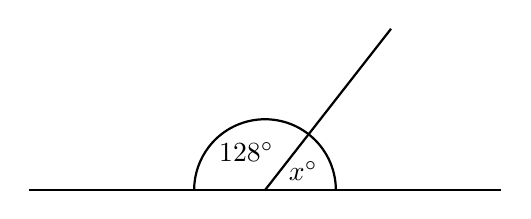
\begin{tikzpicture}[scale=1.0, thick]
        % Points
        \coordinate (A) at (0,0);
        \coordinate (L) at (-3,0);
        \coordinate (R) at (3,0);
        % A ray making 52 degrees with the rightward horizontal
        \path (A) -- ++(52:2.6) coordinate (C);

        % Line and ray
        \draw (L) -- (R);
        \draw (A) -- (C);

        % Angle marks
        % Obtuse angle on the left (128°)
        \pic[draw,angle radius=9mm,"$128^\circ$" {scale=1}] {angle = C--A--L};

        % Acute angle on the right (x°)
        \pic[draw,angle radius=9mm,"$x^\circ$" {scale=1}] {angle = R--A--C};
      \end{tikzpicture}

      \vspace{0.7em}
      Find the value of $x$.
      \ashow{\quad $x = 52^\circ$}

      % ---- Flexible space to push #3 down to align with #4 ----
      \vfill
      \vspace{4em}

      \textbf{3.} \quad $372 + 458 = \ablank{830}$
    \end{column}

    % ===== RIGHT COLUMN =====
    \begin{column}{0.48\textwidth}
      \textbf{2.}

      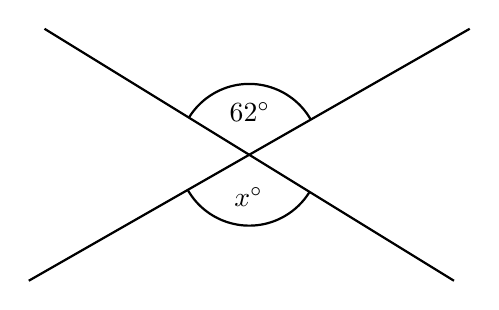
\begin{tikzpicture}[scale=1.0, thick]
        % Intersection point
        \coordinate (O) at (0,0);

        % Two intersecting lines
        \coordinate (A1) at (-2.8,-1.6);
        \coordinate (B1) at (2.8,1.6);
        \coordinate (C1) at (-2.6,1.6);
        \coordinate (D1) at (2.6,-1.6);
        \draw (A1) -- (B1);
        \draw (C1) -- (D1);

        % Mark the top angle as 62°
        \pic[draw,angle radius=9mm,"$62^\circ$" {scale=1}] {angle = B1--O--C1};

        % Mark the vertically opposite (bottom) angle as x°
        \pic[draw,angle radius=9mm,"$x^\circ$" {scale=1}] {angle = A1--O--D1};
      \end{tikzpicture}

      \vspace{0.7em}
      Find the value of $x$.
      \ashow{\quad $x = 62^\circ$}

      % ---- Flexible space to push #4 down to align with #3 ----
      \vfill
        \vspace{1em}
      \textbf{4.} \quad $(84 \div 6) \times 3 = \ablank{42}$
    \end{column}
  \end{columns}

\end{frame}

% ------------------------------------------------------------------
% Worked solutions for Starter 1
% ------------------------------------------------------------------
\begin{frame}
  \frametitle{Worked Solution: Retrieve and Connect 1, Question 1}
  \hypertarget{work-st1}{}

  \textbf{Question:} A ray splits a straight line. One angle is \(128^\circ\), and the other is marked \(x^\circ\). Find \(x\).

  \begin{center}
    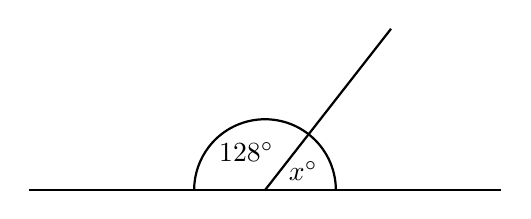
\begin{tikzpicture}[scale=1.0, thick]
      \coordinate (A) at (0,0);
      \coordinate (L) at (-3,0);
      \coordinate (R) at (3,0);
      \path (A) -- ++(52:2.6) coordinate (C);

      \draw (L) -- (R);
      \draw (A) -- (C);

      \pic[draw,angle radius=9mm,"$128^\circ$" {scale=1}] {angle = C--A--L};
      \pic[draw,angle radius=9mm,"$x^\circ$" {scale=1}] {angle = R--A--C};
    \end{tikzpicture}
  \end{center}

  \textbf{Worked Solution:} The two angles lie on a straight line, so their sum is \(180^\circ\). Therefore
  \[
  x + 128^\circ = 180^\circ
  \quad\Rightarrow\quad
  x = 180^\circ - 128^\circ = \ablank{52^\circ}.
  \]
\end{frame}

\begin{frame}
  \frametitle{Worked Solution: Retrieve and Connect 1, Question 2}

  \textbf{Question:} Two straight lines intersect. The top angle is \(62^\circ\), and the vertically opposite angle is marked \(x^\circ\). Find \(x\).

  \begin{center}
    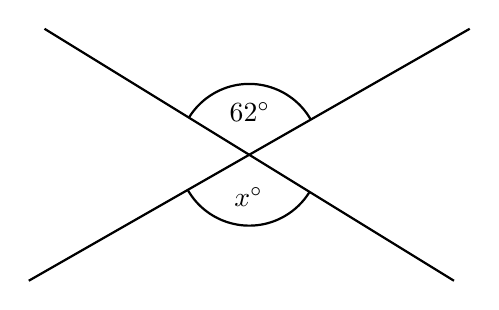
\begin{tikzpicture}[scale=1.0, thick]
      \coordinate (O) at (0,0);
      \coordinate (A1) at (-2.8,-1.6);
      \coordinate (B1) at (2.8,1.6);
      \coordinate (C1) at (-2.6,1.6);
      \coordinate (D1) at (2.6,-1.6);

      \draw (A1) -- (B1);
      \draw (C1) -- (D1);

      \pic[draw,angle radius=9mm,"$62^\circ$" {scale=1}] {angle = B1--O--C1};
      \pic[draw,angle radius=9mm,"$x^\circ$" {scale=1}] {angle = A1--O--D1};
    \end{tikzpicture}
  \end{center}

  \textbf{Worked Solution:} Vertically opposite angles are equal, so
  \[
  x = \ablank{62^\circ}.
  \]
\end{frame}

\begin{frame}
  \frametitle{Worked Solution: Retrieve and Connect 1, Question 3}

  \textbf{Question:} Calculate \(372 + 458\).

  \textbf{Worked Solution:} Add the hundreds, then add the remaining part.
  \[
  372 + 458 = 372 + 400 + 58 = 772 + 58 = \ablank{830}.
  \]
\end{frame}

\begin{frame}
  \frametitle{Worked Solution: Retrieve and Connect 1, Question 4}

  \textbf{Question:} Calculate \((84 \div 6) \times 3\).

  \textbf{Worked Solution:} Work out the division first, then multiply by \(3\).
  \[
  (84 \div 6) \times 3 = 14 \times 3 = \ablank{42}.
  \]
\end{frame}

\end{document}